\documentclass[11pt,a4paper]{article}

\usepackage[T1]{fontenc}
\usepackage[utf8]{inputenc}
\usepackage[brazil]{babel}
\usepackage[margin=2.4cm]{geometry}
\usepackage{amsmath,amssymb}
\usepackage{graphicx}
\usepackage{booktabs}
\usepackage{xcolor}
\usepackage[colorlinks=true,linkcolor=black,urlcolor=blue]{hyperref}
\usepackage{caption}

\captionsetup{font=small,labelfont=bf}
\setlength{\parskip}{0.4em}

\newcommand{\Msun}{M_\odot}
\newcommand{\Req}{R_{\mathrm{eq}}}
\newcommand{\Rpol}{R_{\mathrm{pol}}}
\newcommand{\Btor}{B_\varphi}
\newcommand{\Bpol}{B_{\mathrm{pol}}}
\newcommand{\Etor}{E_{\mathrm{tor}}}
\newcommand{\Epol}{E_{\mathrm{pol}}}

\title{\textbf{Evolução MHD 3D de uma anã branca ultramassiva\\
em rotação diferencial com campo misto}\\[0.3em]
\large Resultados a $192^3$ e $256^3$ --- relatório parcial}
\author{Rafael C.\ R.\ de Lima}
\date{2 de agosto de 2026}

\begin{document}
\maketitle

\begin{abstract}
\noindent
Evoluímos em MHD tridimensional um modelo de equilíbrio de $2{,}005\,\Msun$ com
rotação diferencial forte e campo dominado pela componente toroidal, em duas
resoluções. O resultado central é uma separação: \textbf{a estrela sobrevive e
conserva sua massa, enquanto o campo magnético ordenado é destruído}. Em
$12\,\mathrm{s}$ a energia magnética cai $95\%$ e a razão toroidal/poloidal vai
de $3\times10^5$ a $10$, ao passo que a massa varia $0{,}42\%$ sem tendência. A
instabilidade responsável é não axissimétrica, com $m=1$ dominante, e cresce em
poucos tempos de Alfvén. A taxa de crescimento \emph{não} está convergida: ela
aumenta $47\%$ de $192^3$ para $256^3$, de modo que o valor medido é um limite
inferior. Duas runs seguem em andamento, a $192^3$ já em $t>22\,\mathrm{s}$.
\end{abstract}

%======================================================================
\section{O que está sendo simulado}

\subsection{A configuração}

O objeto é uma anã branca de $M = 2{,}005\,\Msun$, portanto \textbf{38\% acima
do limite de Chandrasekhar} para $\mu_e = 2$ ($1{,}456\,\Msun$). O excesso é
sustentado por rotação diferencial, e essa é a razão física de a estrela ser tão
achatada: $\Req = 3{,}917\times10^8$\,cm contra $\Rpol = 1{,}501\times10^8$\,cm,
ou $\Rpol/\Req = 0{,}383$.

\begin{table}[h]
\centering
\small
\begin{tabular}{lll}
\toprule
Massa & $2{,}0052\,\Msun$ & $1{,}38\,M_{\mathrm{Ch}}$ \\
Densidade central & $3{,}0\times10^{9}$ g\,cm$^{-3}$ & \\
Raios & $\Req = 3{,}917\times10^8$ cm & $\Rpol = 1{,}501\times10^8$ cm \\
Rotação & $\Omega_c = 8{,}193$ rad\,s$^{-1}$ & lei $j$-constante, $A = \Req$ \\
$T/|W|$ & $0{,}0993$ & parâmetro de \emph{shedding} $0{,}469$ \\
Campo toroidal & $\max|\Btor| = 3{,}23\times10^{13}$ G & $0{,}732\,B_c$ \\
Campo poloidal & dipolo de superfície $1{,}0\times10^{9}$ G & \\
Razão de amplitudes & $B_t/B_p = 4234$ & $\Etor/E_{\mathrm{mag}} = 0{,}99999995$ \\
Escalas de tempo & $t_{\mathrm{dyn}} = 0{,}475$ s & $t_A = 2{,}383$ s, $P_{\mathrm{rot}} = 0{,}767$ s \\
\bottomrule
\end{tabular}
\caption{Propriedades do modelo inicial \texttt{rotating\_mixed.txt}.}
\end{table}

A lei de rotação é $j$-constante, $\Omega(\varpi) = \Omega_c A^2/(A^2+\varpi^2)$
com $A = \Req$. Ela é o caso mais diferencial dessa família e deixa a estrela
\emph{marginalmente} estável pelo critério de Rayleigh ($\mathrm{d}j/\mathrm{d}\varpi = 0$).

\subsection{Os campos}

O campo é \textbf{misto, mas dominado pelo toroidal a uma parte em $10^7$ em
energia}. O poloidal existe como um dipolo fraco de $10^9$\,G na superfície;
integrado, $\Epol/|W| = 5{,}2\times10^{-10}$. Essa é a especificação da
colaboração: interior toroidal intenso, dipolo exterior fraco --- e é exatamente
a combinação que um campo puramente toroidal torna instável a Tayler.

\subsection{Equação de estado}

\texttt{ztwd}: gás de elétrons \textbf{completamente degenerado a temperatura
zero}, com $\mu_e = 2$. É \textbf{barotrópica}, $P = P(\rho)$: as derivadas em
temperatura são identicamente nulas e não há capacidade térmica. Isso tem duas
consequências que retomo na Sec.~\ref{sec:ressalvas} --- não existe reservatório
térmico para receber energia dissipada, e a estratificação é neutra, sem empuxo
para limitar instabilidades magnéticas.

\subsection{Método numérico}

\begin{itemize}\itemsep2pt
\item \textbf{Código:} \textsc{Castro} 26.07 sobre AMReX, MHD ideal com
      \emph{constrained transport} (div$\,\mathbf{B}$ preservado por
      construção), Riemann HLLD, PPM desligado.
\item \textbf{Malha:} cartesiana 3D, nível único --- o transporte restrito do
      \textsc{Castro} não faz AMR. Caixa de $1{,}8\times10^9$\,cm de lado,
      idêntica nas duas resoluções.
\item \textbf{Resoluções:} $192^3$ ($\mathrm{d}x = 9{,}375\times10^6$\,cm) e
      $256^3$ ($7{,}031\times10^6$\,cm).
\item \textbf{Gravidade:} \texttt{PoissonGrav}, solução de Poisson 3D completa.
      Não monopolar --- com $\Rpol/\Req = 0{,}38$ o quadrupolo é enorme e uma
      aproximação monopolar faria a estrela ``tocar sino''.
\item \textbf{Condição inicial:} o modelo axissimétrico é construído por
      Grad--Shafranov/SCF numa grade $(\varpi,z)$ de $385\times769$ e
      interpolado para a malha cartesiana a partir do potencial vetor. A
      reconstrução retém $96{,}0\%$ do pico de $|\Btor|$ a $96^3$ e $98{,}9\%$ a
      $192^3$. O campo entra em unidades de Heaviside--Lorentz,
      $\mathbf{B}' = \mathbf{B}/\sqrt{4\pi}$.
\item \textbf{Robustez:} piso de densidade $10^2$\,g\,cm$^{-3}$ contra um
      ambiente de $2{,}0\times10^4$; \emph{sponge} entre $10^4$ e $10^5$;
      amortecimento de velocidade nos primeiros $2\,t_{\mathrm{dyn}}$ dirigido ao
      campo de velocidades \emph{do modelo}, não a zero.
\item \textbf{CFL:} $0{,}5$ no $192^3$; $0{,}3$ no $256^3$ a partir de
      $t \simeq 4{,}8$\,s, necessário para atravessar a saturação.
\end{itemize}

\subsection{Diagnósticos}

Os diagnósticos magnéticos nativos do \textsc{Castro} (\texttt{emag\_density},
\texttt{etor\_density}, \texttt{Div\_B}) mostraram-se inutilizáveis: as três
derivadas empacotam componentes centradas em face de tipos diferentes num único
FAB centrado em célula e leem fora da caixa de dados, com \texttt{Div\_B}
atingindo $3\times10^{146}$ onde deveria ser $\sim0$. As componentes
$B_x, B_y, B_z$ estão corretas, e todos os números aqui foram reconstruídos
delas por ferramentas escritas para isto (\texttt{fbtbp}, \texttt{fmodes},
\texttt{fslice}), com a decomposição
\[
\Btor = \frac{-y\,B_x + x\,B_y}{\varpi}, \qquad
B_{\mathrm{pol}}^2 = B_x^2 + B_y^2 + B_z^2 - \Btor^2 .
\]
Massa e raios são integrados sobre as células com
$\rho > 10^5$\,g\,cm$^{-3}$, ou seja, referem-se à \emph{estrela} e não à caixa.

%======================================================================
\section{Resultados}

\subsection{A estrela sobrevive; o campo, não}

Este é o resultado central e ele se sustenta nas duas resoluções.

\begin{table}[h]
\centering
\small
\begin{tabular}{lrrr}
\toprule
& $t = 0$ & $t = 12$\,s & razão \\
\midrule
Massa da estrela ($\Msun$) & 2{,}00667 & 2{,}00160 & $0{,}9975$ \\
$\Etor$ (erg) & $6{,}035\times10^{49}$ & $2{,}947\times10^{48}$ & $\mathbf{0{,}049}$ \\
$E_{\mathrm{mag}}$ (erg) & $6{,}035\times10^{49}$ & $3{,}078\times10^{48}$ & $0{,}051$ \\
$\Etor/\Epol$ & $3{,}11\times10^{5}$ & $22{,}6$ & \\
$\max|\Btor|$ (G) & $3{,}196\times10^{13}$ & $3{,}539\times10^{13}$ & $1{,}11$ \\
\bottomrule
\end{tabular}
\caption{Estado inicial e final do run a $192^3$. A massa é conservada em
$0{,}42\%$ de amplitude ao longo de toda a série, sem tendência, enquanto a
energia magnética cai por fator 20.}
\end{table}

Note a última linha: \textbf{o campo de pico não cai --- ele sobe 11\%}. O que
desaparece é a organização em grande escala, não a intensidade local. Definindo
um volume efetivo por $V_{\mathrm{ef}} = 8\pi \Etor/\max|\Btor|^2$, a fração da
estrela ocupada pelo campo toroidal cai de $1{,}23\%$ a $0{,}066\%$: um fator 18
de concentração. O campo vira filamento.

\begin{figure}[t]
\centering
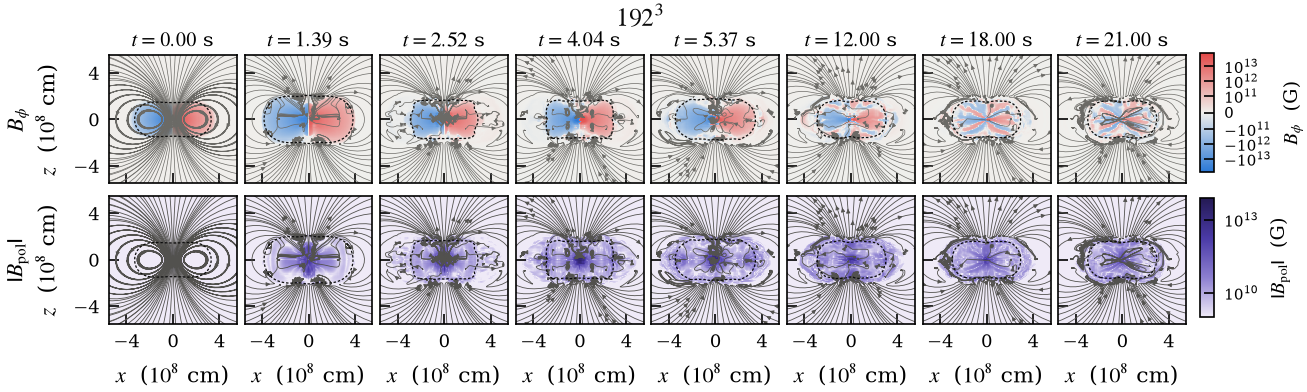
\includegraphics[width=\textwidth]{figures/field_sequence_192.png}
\caption{$192^3$: campo toroidal (cima) e módulo do poloidal (baixo) no plano
meridional $y=0$, onde $B_y$ \emph{é} $\Btor$ e $(B_x,B_z)$ \emph{é} o poloidal.
Linhas: campo poloidal, integradas de $\mathbf{B}$. Tracejado:
$\rho = 10^6$\,g\,cm$^{-3}$. Em $t=0$ os dois lobos de sinal oposto são a
antissimetria $\Btor(x) = -\Btor(-x)$. Escala de cor fixa em todos os painéis e
igual à da Fig.~\ref{fig:seq256}.}
\label{fig:seq192}
\end{figure}

A Fig.~\ref{fig:seq192} mostra o processo. O toroidal parte de dois lobos limpos,
desenvolve estriações radiais em $t \simeq 4$\,s e termina, entre $t = 12$ e
$21$\,s, como um leque de filamentos finos alternando sinal. O poloidal faz o
caminho oposto: nasce como dipolo limpo carregando $10^{-7}$ da energia magnética
e acaba preenchendo a estrela, com linhas emaranhadas além de qualquer função de
fluxo.

\subsection{Densidade, massa, raio e volume}

\begin{figure}[t]
\centering
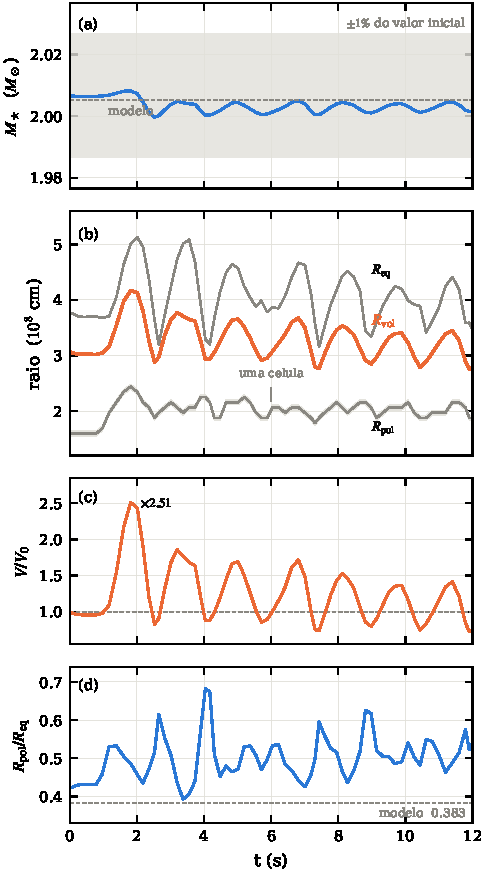
\includegraphics[width=0.62\textwidth]{figures/mass_radius_192.pdf}
\caption{$192^3$ até $t=12$\,s. (a) massa da estrela contra uma faixa de
$\pm1\%$; (b) os três raios, com uma célula de malha desenhada como faixa em
torno de $\Rpol$; (c) volume; (d) oblatidade. O desvio de $\Rpol/\Req$ em $t=0$
--- $0{,}425$ medido contra $0{,}383$ do modelo --- é discretização, não
evolução: $\Rpol$ quantiza em múltiplos de $\mathrm{d}x$ e $\Req$ é cortado pelo
limiar de densidade num perfil equatorial raso.}
\label{fig:massradius}
\end{figure}

A massa fica entre $1{,}99971$ e $2{,}00822\,\Msun$ --- $0{,}42\%$ de amplitude,
sem tendência --- e converge para o valor do modelo, $2{,}00515$, à medida que o
ambiente capturado pelo corte se dissipa. \textbf{A estrela não perde matéria},
apesar de perder $95\%$ da energia magnética.

O que ela faz é pulsar, com amplitude grande: o volume oscila por um fator
$3{,}46$ ao longo do run, com pico em $2{,}51\,V_0$ em $t = 1{,}8$\,s. A
densidade média vai de $1{,}31$ a $4{,}53\times10^{7}$\,g\,cm$^{-3}$. Ao fim de
$12$\,s a estrela está \emph{menor} do que começou ($0{,}74\,V_0$) mas com
densidade central pela metade: ficou consideravelmente \textbf{menos concentrada}
--- a razão $\rho_c/\langle\rho\rangle$ cai de 91 para 34.

\begin{figure}[t]
\centering
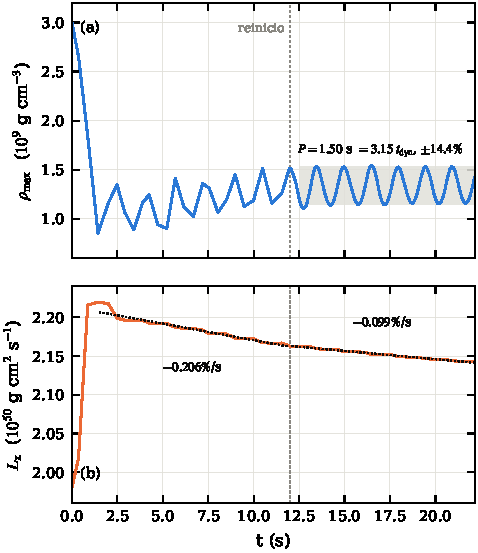
\includegraphics[width=0.62\textwidth]{figures/long_run_192.pdf}
\caption{$192^3$ estendido a $t = 22$\,s (run em andamento). (a) densidade
central; (b) momento angular axial, com as duas taxas de frenagem ajustadas. O
tracejado vertical marca o reinício em $t=12$\,s a partir de \texttt{chk03436};
é um reinício, não uma descontinuidade.}
\label{fig:long}
\end{figure}

Passado o transiente inicial, a pulsação \textbf{não amortece}: ela trava num
modo periódico limpo (Fig.~\ref{fig:long}a) de
\[
P = 1{,}498\ \mathrm{s} = 3{,}15\,t_{\mathrm{dyn}} = 1{,}95\,P_{\mathrm{rot}},
\qquad \text{amplitude } \pm14{,}4\%\ \text{em } \rho_{\max},
\]
com envoltória decaindo em $\sim\!140$\,s. Picos sucessivos: $1{,}531$,
$1{,}530$, $1{,}540$, $1{,}528$, $1{,}530$, $1{,}532$ ($\times10^9$).

\subsection{Evolução dos campos}

\begin{figure}[t]
\centering
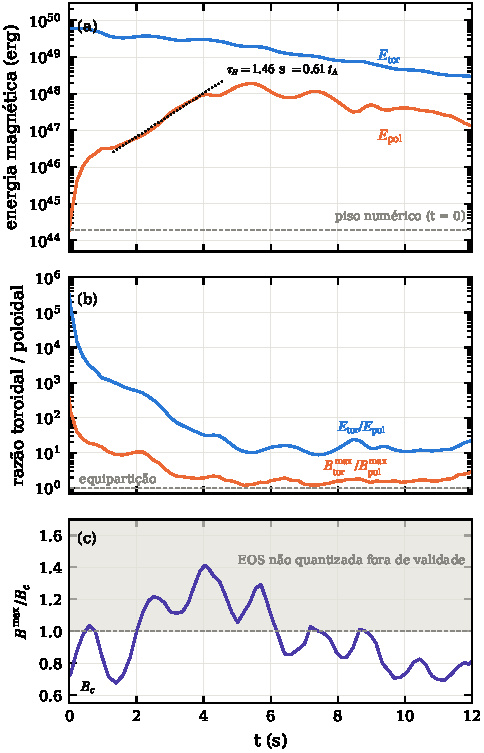
\includegraphics[width=0.62\textwidth]{figures/bt_bp_192.pdf}
\caption{$192^3$ até $t=12$\,s. (a) energias toroidal e poloidal, com o piso
numérico de $\Epol$ em $t=0$ marcado e o ajuste exponencial da fase de
crescimento; (b) as duas razões toroidal/poloidal, em energia e em amplitude de
pico, que saturam em lugares diferentes; (c) campo de pico contra o campo
crítico de Landau.}
\label{fig:btbp}
\end{figure}

O campo passa por três fases distintas (Fig.~\ref{fig:btbp}):

\paragraph{Crescimento, $t = 1{,}3$--$4{,}0$\,s.} A energia poloidal cresce
exponencialmente, $\sigma = 1{,}369$\,s$^{-1}$ com $r = 0{,}994$, partindo de
$1{,}94\times10^{44}$\,erg --- que é o piso de interpolação, não física. O
$e$-folding da \emph{amplitude} é $1{,}46$\,s $= 0{,}61\,t_A$.

\paragraph{Saturação, $t \simeq 5{,}3$\,s.} $\Epol$ atinge
$1{,}88\times10^{48}$\,erg, quase $10^4$ vezes o piso. A razão de amplitudes
$\max|\Btor|/\max|\Bpol|$ chega a $1{,}19$: o poloidal alcança o toroidal em
intensidade de pico. Em energia só chega a $10\%$, porque o toroidal ocupa muito
mais volume --- as duas razões saturam em lugares diferentes e citar uma delas
sozinha descreve mal o estado.

\paragraph{Decaimento, $t > 5{,}4$\,s.} $\Etor$ cai com $e$-folding de
$3{,}44$\,s $= 1{,}44\,t_A$. Em $t = 12$\,s restam $4{,}9\%$ do toroidal
inicial.

\paragraph{A instabilidade é $m=1$.} A decomposição de Fourier azimutal
(ferramenta \texttt{fmodes}, projeção direta sobre células, sem interpolação)
dá, em $t = 0$, $|m{=}1|/|m{=}0| = 1{,}2\times10^{-16}$ --- a condição inicial é
axissimétrica a precisão de máquina. A partir de $t \simeq 2{,}5$\,s
\textbf{o campo poloidal passa a ser dominado por $m=1$}, com
$|B_{z,m=1}|/|B_{z,m=0}|$ chegando a 21 em $t = 4$\,s, enquanto o toroidal
permanece largamente axissimétrico ($m1/m0$ subindo só a $0{,}14$). No estado
final o $m=1$ do toroidal satura em $\simeq 10\%$ do axissimétrico.

Isso exclui a MRI axissimétrica de Balbus--Hawley, que aliás não poderia existir
nesta malha: construído com o campo \emph{vertical}
($B_{\mathrm{pol,rms}} = 7{,}6\times10^8$\,G, $v_{A,\mathrm{pol}} =
3{,}7\times10^4$\,cm\,s$^{-1}$), o comprimento de onda mais instável é
$\lambda_{\mathrm{MRI}} = 2{,}9\times10^4$\,cm, ou $0{,}003$ célula. Restam o
\emph{kink} de Tayler e a MRI não axissimétrica de campo toroidal, ambas $m\ge1$,
que o número de modo azimutal sozinho não separa.

\subsection{Momento angular}

$L_z$ cai a $0{,}206\%$\,s$^{-1}$ enquanto o campo toroidal vive e a
$0{,}099\%$\,s$^{-1}$ depois (Fig.~\ref{fig:long}b) --- \textbf{um fator 2,1 mais
lento assim que $95\%$ da energia magnética se foi}. É a evidência direta de que
o transporte de momento angular era magnético. Ao ritmo atual, mais $10\%$ de
$L_z$ levariam $\sim\!100$\,s.

%======================================================================
\section{Convergência numérica}
\label{sec:conv}

\begin{figure}[t]
\centering
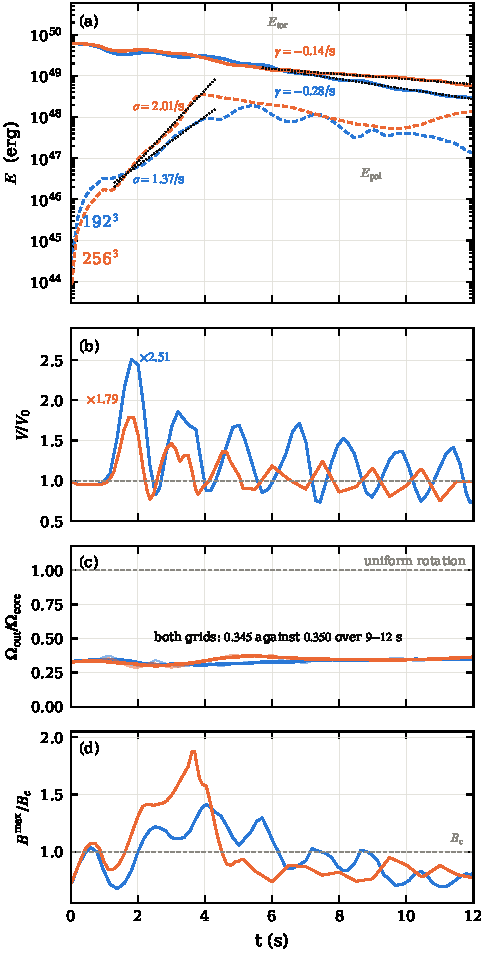
\includegraphics[width=0.62\textwidth]{figures/convergence_192_256.pdf}
\caption{$192^3$ contra $256^3$ na fase de crescimento. (a) energia poloidal com
os ajustes; (b) volume; (c) razão de amplitudes com a equipartição marcada.}
\label{fig:conv}
\end{figure}

\begin{figure}[t]
\centering
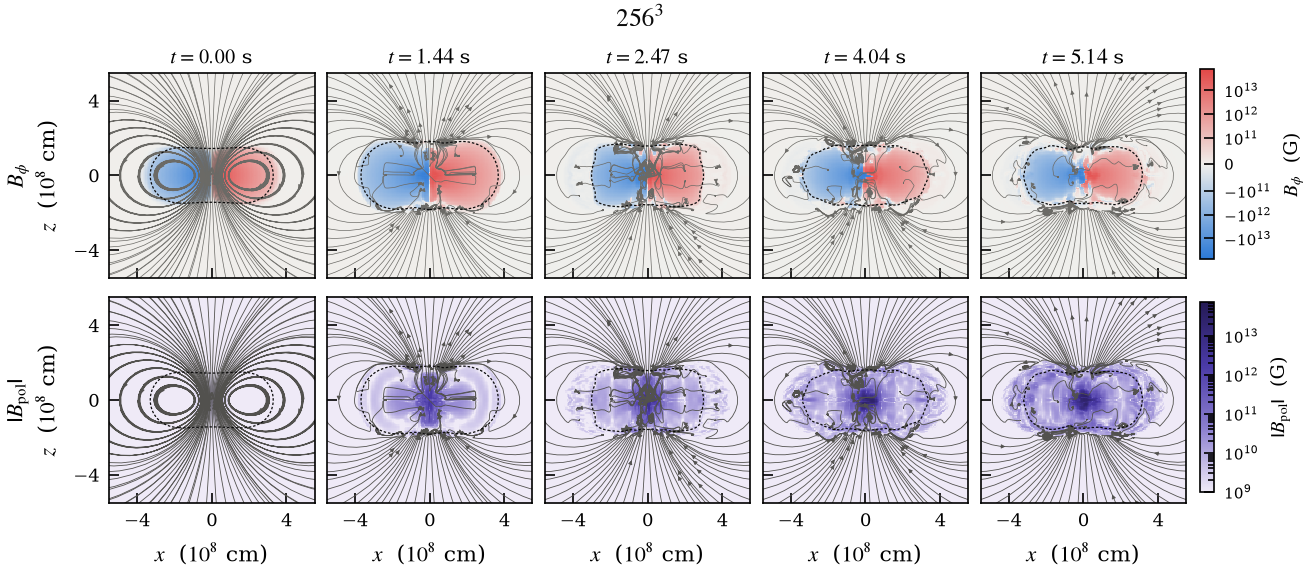
\includegraphics[width=\textwidth]{figures/field_sequence_256.png}
\caption{$256^3$, mesma disposição e mesma escala de cor da Fig.~\ref{fig:seq192},
nos instantes correspondentes.}
\label{fig:seq256}
\end{figure}

Três testes, três veredictos diferentes.

\paragraph{Convergido: massa e volume.} A massa fica em
$1{,}99971$--$2{,}00822\,\Msun$ a $192^3$ e $2{,}00208$--$2{,}00730$ a $256^3$;
o raio equivalente ao volume difere $0{,}03\%$ em $t=0$. Não há figura a fazer.

\paragraph{Não convergido: a taxa de crescimento.} Este é o ponto que precisa
constar de qualquer versão do resultado:
\begin{center}
\small
\begin{tabular}{lccc}
\toprule
& $192^3$ & $256^3$ & razão \\
\midrule
$\sigma$ da energia poloidal & $1{,}369$ s$^{-1}$ & $2{,}007$ s$^{-1}$ & $1{,}47$ \\
$\sigma$ do modo $m=1$ de $\Btor$ & $1{,}968$ s$^{-1}$ & $2{,}752$ s$^{-1}$ & $1{,}40$ \\
$\Epol(t=0)$, o piso numérico & $1{,}94\times10^{44}$ & $1{,}16\times10^{44}$ & $0{,}60$ \\
$\min(\max|\Btor|/\max|\Bpol|)$ & $1{,}19$ & $\mathbf{0{,}805}$ & \\
\bottomrule
\end{tabular}
\end{center}
A taxa \emph{sobe} $47\%$ com a resolução, medida por dois diagnósticos
independentes que concordam no fator, e a malha fina parte de uma semente
\emph{menor}. Ela também leva a instabilidade mais longe: o poloidal ultrapassa
o toroidal em pico a $256^3$ e nunca o faz a $192^3$. \textbf{O $\sigma$ medido
é um limite inferior}, e o mesmo vale para a intensidade da instabilidade.

\paragraph{Numérico: a pulsação inicial.} O primeiro pico de volume cai de
$2{,}51\,V_0$ a $1{,}79$ e o segundo de amplitude $0{,}49$ a $0{,}11$
(Fig.~\ref{fig:conv}b). O ``respirar'' que domina os primeiros segundos é em boa
parte a condição inicial ressoando na malha. O modo persistente de $1{,}50$\,s
que aparece depois de $t=12$\,s é outro fenômeno, e ainda não foi testado em
resolução.

Uma observação de custo: fechar a taxa exigiria $384^3$, cerca de cinco vezes o
custo do $256^3$. O caminho alternativo --- e provavelmente o correto --- é
introduzir resistividade explícita, dando ao problema uma escala de dissipação
física em vez de deixar a malha defini-la. O \textsc{Castro} não a implementa
hoje.

%======================================================================
\section{Ressalvas}
\label{sec:ressalvas}

\begin{enumerate}\itemsep3pt
\item \textbf{A EOS é barotrópica.} Com \texttt{ztwd} não há reservatório
      térmico: os $5{,}7\times10^{49}$\,erg que saem do campo não têm destino
      físico e são dissipados na escala da malha. Podemos afirmar que o campo
      ordenado é destruído; não podemos dizer para onde a energia foi nem quanto
      aquecimento isso causaria. A estratificação também é neutra, sem empuxo
      para limitar o modo --- numa estrela estratificada a taxa seria menor, o
      que reforça a leitura de $\sigma$ como limite superior \emph{físico} ao
      mesmo tempo que é limite inferior \emph{numérico}.
\item \textbf{Parte do run está fora da faixa de validade da EOS.} O campo de
      pico atinge $1{,}41\,B_c$ em $t = 4{,}0$\,s e fica acima do campo crítico
      de Landau em $44\%$ dos instantes amostrados. A \texttt{ztwd} supõe gás não
      quantizado.
\item \textbf{Tayler contra MRI toroidal não está resolvido.} Ambas são $m\ge1$.
      O caso não rotante do trabalho companheiro não ajuda a decidir: lá a
      estrela colapsa radialmente em $2{,}5$\,s, pela coluna axial onde
      $\Btor$ se anula, e o modo não axissimétrico nunca é alcançado. Comparado
      a ele, o presente resultado é que \textbf{a rotação troca um destino por
      outro}: a estrela deixa de colapsar e passa a perder o campo.
\end{enumerate}

%======================================================================
\section{Situação das simulações}

\begin{itemize}\itemsep2pt
\item \textbf{$192^3$ estendido} (\texttt{wdrot192long}): em execução, já além de
      $t = 22$\,s, alvo $60$\,s. O passo de tempo quadruplicou desde $t=12$\,s
      conforme o campo morreu, então deve chegar bem antes das nove janelas
      orçadas.
\item \textbf{$256^3$} (\texttt{wdrot256}): em execução, $t \simeq 7{,}3$\,s de
      $12$. Atravessou com CFL $0{,}3$ o ponto $t = 5{,}146$\,s onde duas
      tentativas anteriores abortaram deterministicamente.
\end{itemize}

Tudo --- \emph{inputs}, \emph{scripts} de submissão, ferramentas de diagnóstico,
dados e código das figuras --- está versionado no repositório \texttt{WD\_MAG}.

\end{document}
